% This is a template for use with the MSU Thesis class
% Version 3.6 2022/08/23
%
% Class options: 
%[PhD]	Doctor of Philosophy (default) 
%[DEd]	Doctor of Education
%[DMA]	Doctor of Musical Arts
%[DNP]	Doctor of Nursing Practice
%[MA]	Master of Arts
%[MS]	Master of Science
%[MAT]	Master of Arts for Teachers
%[MBA]	Master of Business Administration
%[MFA]	Master of Fine Arts
%[MIPS]	Master of International Planning Studies
%[MHRL]	Master of Human Resources and Labor Relations 
%[MMus]	Master of Music
%[MPH]	Master of Public Health
%[MPP]	Master of Public Policy
%[MSW]	Master of Social Work
%[MURP]	Master in Urban and Regional Planning 
%%
% Default is PhD
%
%
% This template has everything in the right order.
% Just add real content and you're done!
%
\documentclass[]{msu-thesis}
%
% for a prettier, but possibly non-compliant table of contents use the [mixedtoc] option
% for a plain table of contents use the [plaintoc] option
% for a horrendous looking, but possibly required table of contents, use the [boldtoc] option
%
% If you have large tables/figures that need to be in landscape mode, add the [lscape] option
%
% The class accepts 12pt, 11pt or 10pt font size options. 
% For Times New Roman as in this example document, use 12pt (default).
%
\usepackage{amsmath}
\usepackage{csquotes}
\usepackage{float}
\usepackage{hyperref}
% \usepackage[document]{ragged2e}
\usepackage{graphicx}
\usepackage{caption}
\usepackage{subcaption}
%\usepackage{multirow,ragged2e}
%\usepackage{ragged2e}
\usepackage{tikz-cd}
\usepackage[final]{pdfpages}
\usepackage[
backend=biber,
style=numeric-comp,
sorting=none
]{biblatex}
\addbibresource{bibliography.bib}
% If you require per-chapter appendices add the [chapterapp] option
%
% If you require per-chapter bibliographies add the [chapterbib] option
%
% This is standard fontenc for pdflatex
% If you use LuaLaTeX or XeLaTeX you should replace this with the fontspec package
\usepackage[T1]{fontenc}
%
% If the thesis office requires Times, we'll give them Times
% You can experiment with other font packages here if you like.
% If you are using XeLaTeX or LuaLaTeX load  TeX Gyre Termes, Times or Times New Roman font with \setmainfont
\usepackage{newtxtext,newtxmath} 
%
% Load any extra packages here
%
% You must specify the title of your thesis, your name, the field of study (not department), and the year
\title{Resonance Compensation Studies at the FNAL Recycler Ring}
\author{Cristhian Gonzalez-Ortiz}
\fieldofstudy{Physics} % This should be in sentence case
\date{2024}

% If you want a dedication page, specify the text of the dedication here and uncomment the next command.
%
%\dedication{This thesis is dedicated to someone.}
%
\begin{document}

% All the stuff before your actual chapters is called the front matter
\frontmatter
% First make the title page
\maketitlepage

% if you have public abstract (optional) it should go here
%\begin{publicabstract}
% Public abstract goes here
%\end{publicabstract}

% Next make the regular abstract (obligatory)
\begin{abstract}
% Your abstract goes here.  Master's 1 page max. PhD 2 page max.
Circular accelerators, such as the ones in the Fermilab Accelerator Complex, are indispensable tools driving scientific discovery by propelling particles to high energies and high intensities. In the context of the Proton Improvement Plan II (PIP-II) at Fermilab, the Recycler Ring (RR) is confronted with the challenge of high-intensity operation. The space charge tune shifts at these intensities necessitate the mitigation of third-order resonances. By measuring the Resonance Driving Terms (RDTs) for each resonance line, their strengths and damaging effects can be quantified. 

The study is focused on the utilization of dedicated normal and skew sextupoles for the compensation of these resonance lines. By employing the response matrix method to measure the Resonance Driving Terms (RDTs) relative to the currents in these sextupoles, a methodical approach to simultaneously compensate individual and multiple third-order resonances has been developed and assessed. The assessment and verification incorporate mapping out beam losses through dynamic and static tune scans, along with the utilization of the Ion Profile Monitor (IPM) system for beam size measurements. 

Furthermore, optimization algorithms have been explored and incorporated into the resonance compensation scheme. Parallel, to the work done at Fermilab, the study extends its scope by performing related experiments at the CERN Proton Synchrotron Booster (PSB). For these experiments, multiple resonance lines in the tune diagram were compensated by optimizing the currents in the compensation elements with the aid of advanced optimization algorithms.  

High-intensity operation of the Recycler Ring involves understanding the interplay between the space charge tune spread, resonance lines, and specialized subsystems such as transverse dampers. The following study also delves into experiments that try to discern each of these phenomena, while highlighting challenges still ahead. Overall, these studies indicate the feasibility of compensating for multiple third-order resonances, contributing to the objectives of PIP-II for the reliable delivery of a 1.2 MW proton beam to experimental facilities.
\end{abstract}

% Force a newpage
\clearpage
% Make the copyright page. The Graduate School ridiculously claims that you
% can't have a copyright page unless you pay ProQuest to register the copyright.
% This is simply not the case, so put in your copyright page whether or not you
% intend to pay Proquest to register the copyright.
% Furthermore, they have occasionally complained that the copyright mark is aligned
% to the right, even though that has been the format for more than a decade.
% If they want the copyright mark aligned to the left, use \makecopyrightpage* instead. 

\makecopyrightpage 

% If you have a dedication page, uncomment the next command to print the dedication page
%
%\makededicationpage
%
\clearpage
% Your Acknowledgements are formatted like a chapter, but with no number
\chapter*{Acknowledgements}
\DoubleSpacing % Acknowledgements should be double spaced
I would like to acknowledge Dr. Robert Ainsworth for taking those couple of nutmegs when we played footy together. Thank you, Rob, for making me a better scientist and teaching me so many valuable life lessons. Thank you for always having my back.

I would like to acknowledge the instrumental role of Dr. Peter Ostroumov in these years of my Ph.D. at Michigan State University. Thank you, Peter, for pushing me to be a better physicist and scientist, every day. Thank you for believing in me, even in the moments I didn't believe in myself.

Thank you to the members of my doctoral committee, Steve Lund, Yue Hao, Paul Gueye and Kendall Mahn. I truly value every comment and every word of encouragement at all of our meetings. We did not meet frequently, but your guidance was crucial through this process. Also thank you to whole support network at MSU and FRIB---these are institutions where you will never feel alone and always have someone support you when needed.

I would like to acknowledge the whole MI/RR department at Fermilab. Thank you, Kyle, Adam, Nino, Osama, Betiay, Denton, Marty, Mike, Phil, MaryKate, Matilda and Meiqin, and whoever I might have left out. Thank you for having the patience and your unconditional support while I pushed through with my experiments. You guys always had a smile even when I asked the most basic questions. Special acknowledgement to the operations team at Fermilab for always being open to questions and discussion. Thank you for having the patience to withstand me when I would continuously trip the permit on beam losses. I would also like to acknowledge the hospitality and awesomeness of our CERN collaborators, specially Foteini and Tirsi. 

Luisa. Tú has sido el soporte y la inspiración estos últimos años para poder estar a puertas de cruzar la meta. Gracias por siempre estar ahí y no rendirte nunca con lo nuestro. Vamos a lograr grandes cosas juntos. Ya casi adoptamos un perrito, manguitos szah.

Gracias a toda mi familia, incluyendo a esos amigos que considero mi familia, por apoyarme en este camino. Desde Bogotá hasta llegar a Chicago pasando por Lansing. Nunca pensé en llegar tan lejos de la loma. No hubiera podido terminar este doctorado sin el apoyo de todos ustedes. Gracias por estar ahí en cada momento de mi vida. Thank you, Sjuju, the great celestial whale overseer.

%
\clearpage
% We need to turn single spacing back on for the contents/figures/tables lists
\SingleSpacing
\tableofcontents* % table of contents will not be listed in the TOC
%\clearpage
%\listoftables % comment this out if you have no tables
%\clearpage
%\listoffigures % comment this out if you have no figures
%
% If you have a Key to  Abbreviations/symbols you would add each abbreviation in its display order
% using as in the following examples:
\abbrev{MSU}{Michigan State University}
\abbrev{FNAL}{Fermilab National Accelerator Laboratory}
\abbrev{RR}{Recycler Ring}
\abbrev{MI}{Main Injector}
\abbrev{RDTs}{Resonance Driving Terms}
\abbrev{NuMI}{Neutrinos at the Main Injector}
\abbrev{PSB}{CERN Proton Synchrotron Booster}
\abbrev{ACNET}{Accelerator Control Network}
\abbrev{TbT}{Turn-by-Turn Data}
\abbrev{NAFF}{Numerical Analysis of Fundamental Frequencies}
\abbrev{GFCs}{Generating Function Coefficients}
% Then issue a \clearpage and print the list 
\clearpage
\listofabbreviations 
% Comment out the code above if you have no abbreviations
% See the documentation if you need to change the width or format of the abbreviation column

% See the class documentation and the Memoir manual for how to create other lists
%
% If you are using an algorithm formatting package (e.g. algorithmicx or algorithm2e)
% please read the class documentation carefully on how to use these packages with the class
% The class provides an {algorithm} environment and a \listofalgorithms by default 
%
\mainmatter
%
% The next line removes the dots in chapter headings in the TOC
% May violate thesis office rules
%\addtocontents{toc}{\protect\renewcommand{\protect\cftchapterdotsep} {\cftnodots}}

% ALL documents using this class must have \chapter divisions
% If you are using it for an MA/MS thesis you still need to have chapters, even if they are very small.
\chapter{Introduction}
\label{sec:ch1}
 
Particle accelerators are the workhorses for modern scientific discoveries. Experimental nuclear and particle physics research benefit greatly from the progress of accelerator physics and technology. Accelerator physics is a rich field of applied physics living on the intersection of electromagnetism, solid-state and atomic physics, nonlinear mechanics, plasma physics, quantum mechanics, just to name a few \cite{sylee}. Furthermore, the design and operation of modern accelerator projects require costly enterprises of scientists, engineers, operators, and politicians coming together under one single metaphorical roof.         

\section{Circular Accelerators and Storage Rings}

As will become more apparent on Ch. \ref{sec:ch2}, a particle accelerator can be thought of as a composition of accelerator-themed LEGO® bricks \cite{forest}. Each elemental LEGO® brick can be thought of as an accelerator component performing some mapping on the charged particles entering it. As it turns out, these LEGO® bricks can be assembled together in a circular fashion to give rise to circular accelerators. For the case where particles are not accelerated on these structures, a storage ring arises.     

\section{Fermilab}

The Fermi National Accelerator Laboratory (FNAL), better known as Fermilab, has a long and rich history of designing, building and operating high-energy particle accelerators. Ever since the founding director of Fermilab, Robert R. Wilson, envisioned the 400 GeV Main Ring back in 1967, Fermilab has been at the forefront of accelerator physics.     \cite{tevatron},\cite{fermilab1}

\section{Outline}

The following thesis will explore the compensation of third-order resonances in the Fermilab Recycler Ring. This \hyperref[sec:ch1]{first chapter} introduces the motivation behind this thesis work. The \hyperref[sec:ch2]{second chapter} summarizes single particle dynamics with the help of exponential Lie operators and moves forward to introduce a relevant concept of collective beam dynamics: the space charge tune shift. This theoretical overview gives segue into the \hyperref[sec:ch3]{third chapter} of this thesis, where the Recycler Ring is introduced and described in detail. Motivation for the compensation of third order resonances is given in this chapter under the framework of current and future operation of the RR. With the basic physics concepts and the description of the machine put in place, the \hyperref[sec:ch4]{fourth chapter} describes in full detail the scheme and experiments developed in order to compensate third order resonances at low intensities. Before moving to explore the Recycler Ring at high intensities, \hyperref[sec:ch5]{chapter five} provides an interlude in order to show a series of experiments done at the CERN PS Booster. These experiments explore the use of advanced optimization algorithms in the aid of compensating multiple resonance lines simultaneously. Coming back to Fermilab, \hyperref[sec:ch6]{chapter six} showcases the studies and experiments done at high intensities in the RR in order to understand the interplay between the compensation of resonance lines and space charge effects. Finally, \hyperref[sec:ch7]{chapter seven} brings down the curtain by providing some general conclusions and future work stemming from this thesis.
\chapter{Beam Dynamics in Rings}
\label{sec:ch2}

\section{\label{sec:lie}Lie Maps in Accelerator Physics}

The most basic element of a particle accelerator can be thought of as a black box. This black box takes some single charged particle with initial transverse coordinates $\left( x_0,x'_0,y_0,y'_0 \right)$, as defined in a Frenet-Serret coordinate system, and maps them to some final coordinates $\left( x_f,x'_f,y_f,y'_f \right)$. For simplicity, any longitudinal effect will not be taken into account for this analysis, but can be easily incorporated. By gathering the initial coordinates into a vector, i.e. $\vec{X_0} = \left( x_0,x_0',y_0,y_0' \right)$, and doing the same for the final coordinates, i.e., $\vec{X_f} = \left( x_f,x_f',y_f,y_f' \right)$, one can define the mapping $\mathcal{M}$ that relates both vectors, such that:  
\begin{equation}
\label{eq:ch2map}
\vec{X_f}=\mathcal{M}\vec{X_0}.
\end{equation}
For a charged particle inside some accelerator element that can be described using Hamiltonian dynamics, the mapping $\mathcal{M}$ can be understood in terms of Poisson brackets and exponential Lie operators \cite{wolski,todd1,cernthesis1,cernthesis2}.\\
Let $\vec{X} = \left( q_1,p_1,\dots,q_{n},p_{n} \right)$ be a 2n dimensional vector, made from $n$ pairs of canonical coordinates $(q_i,p_i)$ that make up the 2$n$ dimensional phase space. And let two arbitrary functions $f\left( \vec{X};s\right)$ and $g\left( \vec{X};s\right)$ be functions of $\vec{X}$ and $s$, where $s$ plays the role of the independent "time" coordinate. The Poisson brackets $\left[ \bullet , \bullet \right]$ can be defined as:
\begin{equation}
    \label{eq:ch2poisson}
    \left[ f,g \right] = \sum_{i=1}^{n} \frac{\partial f}{\partial q_i}\frac{\partial g}{\partial p_i} - \frac{\partial f}{\partial p_i}\frac{\partial g}{\partial q_i}. 
\end{equation}
Using this definition, one can explicitly write out the Poisson bracket definition for a 4 dimensional phase space described by state vector $\vec{X} = \left( x,x',y,y' \right)$. This reads: 
\begin{equation}
    \label{eq:ch2poisson1}
    \left[ f,g \right] = \frac{\partial f}{\partial x}\frac{\partial g}{\partial x'} - \frac{\partial f}{\partial x'}\frac{\partial g}{\partial x} + \frac{\partial f}{\partial y}\frac{\partial g}{\partial y'} - \frac{\partial f}{\partial y'}\frac{\partial g}{\partial y}. 
\end{equation}\\
The Lie operator $:f:$ acts on some function $g$ and is the adjoint operator of the Poisson bracket operator. Its definition reads:
\begin{equation}
    \label{eq:ch2lie1}
    :f:g = \left[ f,g \right].
\end{equation}
This specific $:\bullet:$ notation allows for a compact notation in order to define the exponential Lie operator. The exponential Lie operator of an arbitrary function $f$ is defined as
\begin{equation}
    \label{eq:ch2explie1}
    e^{:f:}\bullet = \sum_{k=0}^{\infty}\frac{1}{k!}\left( :f: \right)^k \bullet.
\end{equation}
It turns out that for a Hamiltonian system, the mapping of coordinates from $\vec{X_0}$ to $\vec{X_f}$ follows the expression:
\begin{equation}
    \label{eq:ch2liemap1}
    \vec{X_f}=e^{-\ell :H:}\vec{X}\bigg\rvert_{\vec{X}=\vec{X_0}},
\end{equation}
which is known as a Lie Map \cite{todd1}. In this case, $\ell$ corresponds to the integration length of the independent coordinate. For example, for a particle traversing a magnet which has length $L$, the integration length is $\ell = L$. When looking at the one-turn map, the integration length corresponds to the circumference $C$ of the accelerator over an effective Hamiltonian $H_{eff}$. Furthermore, if working with action-angle variables, the integration length $\ell$ would just be the phase advance $\mu$.\\ 

\section{\label{sec:oneturn}One-turn Map and Normal Form}

The one-turn map $\mathcal{M}_1$ of a circular accelerator is the composition ($\circ$) of mappings from every element in the ring. Choosing an arbitrary initial point at $s=0$ and going around the ring, the one-turn map describes the transformation of coordinates after one turn, i.e., $\vec{X}_{N=1}=\mathcal{M}_1 \vec{X_0}$. This map composition reads:
\begin{equation}
    \label{eq:oneturnmap}
    \mathcal{M}_1=M_{N+1} \circ e^{:h_N:} \circ \dots \circ e^{:h_2:} \circ M_2 \circ e^{:h_1:} \circ M_1 = M_{N+1}e^{:h_N:} \dots e^{:h_2:}M_2 e^{:h_1:}M_1,
\end{equation}
where $M_i$ is the matrix representation of a linear mapping, that does not couple $x-y$ plane, e.g., drift space mapping, quadrupole mapping. On the other hand, the map $e^{:h_i:}$ represents any linear or non-linear mapping that can be found around the machine and can be considered a perturbation to the ideal lattice including coupling elements, e.g., skew quadrupoles, higher order multipole elements. Figure \ref{fig:oneturn} illustrates the procedure to build the one-turn map for a circular accelerator. 

\begin{figure}[H]
    \centering
    \includegraphics[width=0.7\columnwidth]{chapter2/oneturn.png}
    \caption{Diagram of an arbitrary circular accelerator in order to illustrate the one-turn map.}
    \label{fig:oneturn}
 \end{figure}

Through the use of the Baker-Campbell-Hausdorff formula , Eq. \ref{eq:oneturnmap} can be collapsed to the expression 
\begin{equation}
    \label{eq:oneturnmapeff}
    \mathcal{M}_1=e^{-C :H_{eff}:},
\end{equation}
where $C$ is the circumference of the ring and $H_{eff}$ is the effective Hamiltonian of the machine over one turn. As mentioned earlier, for most cases, it is of interest to look at the perturbations to the linear uncoupled dynamics of the design lattice. With this in mind, Eq. \ref{eq:oneturnmapeff} can be rewritten as:
\begin{equation}
    \label{eq:oneturnmapeff1}
    \mathcal{M}_1=e^{:h:}R,
\end{equation}
where $R$ is a rotation matrix encoding the linear uncoupled dynamics of the ideal lattice. On the other hand, the term $e^{:h:}$ encodes the perturbations to this ideal situation. It is worth pointing out that for the case $h=0$, the traditional Courant-Snyder variables are recovered.   

The Courant-Snyder variables ($\hat{x}$,$\hat{p}_x$,$\hat{y}$,$\hat{p}_y$) or normalized phase space coordinates can be written for a linear uncoupled case as:
\begin{equation}
    \label{eq:norm1}
    \hat{u}=\sqrt{2J_u} \cos \left( \phi_u + \phi_{u_0}\right);
\end{equation}
\begin{equation}
    \label{eq:norm2}
    \hat{p}_u=-\sqrt{2J_u} \sin \left( \phi_u + \phi_{u_0}\right),
\end{equation}
where $u$ can stand either for the $x$ or $y$ coordinate, $J_u$ and $\phi_u$ correspond to the action-angle variables and $\phi_{u_0}$ corresponds to the initial phase. For the case where perturbations exist, i.e., $h \neq 0$, the action $J_u$ is not constant anymore and will be a function of $\phi_u$.  

The Normal Form formalism is introduced at this point in order to find amplitude-independent coordinates $I_u$ and $\psi_u$, such that the motion just depends on $\psi_u$ at a constant $I_u$, with some initial phase $\psi_{u_0}$. These are known as non-linear action-angle variables. The variables $I_u$ and $\psi_u$ are calculated from the transformation $e^{-:F:}$ acting on $J_u$ and $\phi_u$. Without loss of generality, the generating function $F$ can be written as a Fourier expansion over the objective space $(I_x,\psi_x,I_y,\psi_y)$ such that:
\begin{equation}
    \label{eq:F}
    F=\sum_{jklm} f_{jklm} \left( 2 I_x\right)^{\frac{j+k}{2}} \left( 2 I_y\right)^{\frac{l+m}{2}} e^{i\left[ \left( j-k \right)\left( \psi_x+\psi_{x0} \right)+ \left( l-m \right) \left( \psi_y+\psi_{y0} \right)\right]}.
\end{equation}
In a similar fashion, the argument of the Lie operator $e^{:h:}$ from Eq. \ref{eq:oneturnmapeff1} can be expanded as:
\begin{equation}
    \label{eq:h}
    h=\sum_{jklm} h_{jklm} \left( 2 J_x\right)^{\frac{j+k}{2}} \left( 2 J_y\right)^{\frac{l+m}{2}} e^{i\left[ \left( j-k \right)\left( \phi_x+\phi_{x0} \right)+ \left( l-m \right) \left( \phi_y+\phi_{y0} \right)\right]}.
\end{equation}
For Eqs. \ref{eq:F} and \ref{eq:h}, the integer indices $j,k,l,m$ run from $0$ to infinity, and correspond to the four degrees of freedom for transverse phase space.   

The terms $f_{jklm}$ are known as generating function coefficients. The terms $h_{jklm}$ are known as Hamiltonian coefficients or resonance driving terms (RDTs). Section \ref{sec:rdts} will take a closer look into how RDTs can be used to characterize the non-linear dynamics of accelerators. The generating function coefficients $f_{jklm}$ can be related to the Hamiltonian resonance driving terms $h_{jklm}$ through the following relation \cite{cernthesis1,bartolini}:
\begin{equation}
    \label{eq:handf}
    f_{jklm}=\frac{h_{jklm}}{1-e^{2\pi i \left[ \left( j-k \right) Q_x + \left( l-m\right) Q_y \right] }},
\end{equation}
where $Q_x$ and $Q_y$ represent the transverse uncoupled and unperturbed tunes of the accelerator. The transverse tunes of a circular accelerator are defined as the phase advances in each plane over one turn, in units of $2\pi$, i.e., $Q_u=\phi_u(s=C)/2\pi$. 

\section{Resonances in Circular Accelerators}

Equation \ref{eq:handf} diverges for when the denominator goes to zero. Specifically, this happens when the following condition is met:
\begin{equation}
    \label{eq:resonances}
    \left( j-k \right) Q_x + \left( l-m\right) Q_y = p,
\end{equation}
where $p$ can be any integer. Equation \ref{eq:resonances} defines resonance lines in tune space of order $n=j+k+l+m$. If the accelerator is tuned to operate on top of these resonances, the perturbations will add up coherently turn to turn and kick the resonant particles out of their original trajectory. In general, operating close or on top of a resonance line is harmful as particles will be lost. This is specially true for lower order resonances, i.e., for $n<4$. In general, the higher order of a resonance, the weaker it is \cite{Wiedemann2015}. This thesis work focuses on third order resonances, i.e., $n=3$, and how to mitigate their deleterious effect. 

Figure \ref{fig:tunediagram} shows the tune diagram with resonance lines, as defined by Eq. \ref{eq:resonances}, drawn up to fifth order. The integer part of both tunes are chosen to include the actual area of operation of the Recycler Ring. The operation and tune diagram for the Recycler Ring are described in more detail in Ch. \ref{sec:ch3}. Normally, the operation point of a circular accelerator is chosen to be clear of any resonance line and far away as possible from integer ($n=1$) and half integer ($n=2$) resonances. Nevertheless, in reality there are two concepts that complicate things. The first one relates to the fact that resonance lines are not infinitely thin and have some stop band width. The second one, concerns the fact that at high intensities particles will not have localized tunes, but rather a distribution of tunes with some tune spread, i.e., tune footprint. Section \ref{sec:sc1} takes a closer look at this effect known as space charge tune shift. Ultimately, choosing the operation point on Fig. \ref{fig:tunediagram} is a matter of localizing a resonance-free region where the intensity-dependent tune footprint can be placed.   
\begin{figure}[H]
    \centering
    \includegraphics[width=0.8\columnwidth]{chapter2/tunediagram.png}
    \caption{Tune diagram with resonance lines up to fifth order, enclosing the operation point of the Recycler Ring.}
    \label{fig:tunediagram}
 \end{figure}

 \begin{figure}[H]
    \centering
    \includegraphics[width=\columnwidth]{chapter2/rrtdlow.png}
    \caption{Approximate operational tune footprint at low intensities, i.e., 1e10 particles per bunch.}
    \label{fig:rrtdlow}
 \end{figure}

\section{\label{sec:rdts}Resonance Driving Terms} 

As it turns out, the RDTs $h_{jklm}$ are related to the strength 

The resonance basis can be built by getting the quantity $h_u^{\pm}=\hat{u}\pm \hat{p_u}$ in terms of the number of turns $N$ . Specifically, for $h_x^{-}$ this reads:
\begin{multline}
    \label{eq:hx-}
    h_x^{-}(N)=\sqrt{2I_x}e^{i\left( 2\pi Q_x N +\psi_{x_0}\right)} \\
    -2i \sum_{jklm} j f_{jklm} \left( 2I_x \right)^{\frac{j+k-1}{2}}\left( 2I_y \right)^{\frac{l+m}{2}}
    e^{i \left[ \left( 1-j+k\right)\left( 2\pi Q_x N + \psi_{x_0} \right) +\left( m-l\right)\left( 2\pi Q_y N + \psi_{y_0} \right)\right]},
\end{multline}
where $Q_x$ and $Q_y$ are the horizontal and vertical tune~[3]. 

In general, RDTs are defined by the order in which they enter the one-turn normal form Hamiltonian \cite{bartolini}. The general expression to define RDTs reads:
\begin{equation}
    \label{eq:rdt1}
    h_{jklm}=\Xi _{jklm} \sum_i L_i \beta_{xi}^{\frac{j+k}{2}} \beta_{yi}^{\frac{l+m}{2}} V_{ni}e^{i\left[ (j-k)\phi_{xi} +(l-m) \phi_{yi} \right]},
\end{equation}
where $\Xi _{jklm}$ is just a constant defined as:
\begin{equation}
    \label{eq:rdt2}
    \Xi _{jklm} = -\frac{q}{p_0}\frac{1}{2^n}\frac{1}{n} {\binom{n}{l+m}} {\binom{j+k}{j}}{\binom{l+m}{l}}.
\end{equation}

For Eqs. \ref{eq:rdt1} and \ref{eq:rdt2}, $n=j+k+l+m$ represents the order of the resonance. The sum over $i$ is done over all multipoles of order $n$ and length $L_i$ that either have a normal component $V_{ni}=B_{ni}$ if $l+m$ is even, or a skew component $V_{ni}=A_{ni}$ if $l+m$ is odd. The symbols for $\beta_{xi}$, $\beta_{yi}$, $\phi_{xi}$ and $\phi_{yi}$ represent the beta functions and phase advances in each plane, respectively.

\section{\label{sec:sc1}Space Charge Tune Shift}

\chapter{The FNAL Recycler Ring}
\label{sec:ch3}

\section{\label{sec:intro31}Introduction}
The Fermilab Recycler Ring (RR) is one of the circular accelerators located in the Fermilab Accelerator Complex. It was originally designed to store and accumulate antiprotons that remained from a Tevatron event \cite{rr0}. The recycling of antiprotons was deemed ineffective and was never operationally implemented \cite{rrnagaitsev}. Since 2011, the RR has been repurposed to act as a pre-injector to the Main Injector (MI) by storing and accumulating protons \cite{rr1}. It is worth pointing out, that the MI and the RR share the same tunnel, which has a circumference of 3.319 km (2.062 mi). The work done for this thesis focuses on the Recycler Ring. The following chapter starts by giving a general description for the operation and physics of the Recycler Ring. The next sections introduce and motivate the compensation of third order resonances for high intensity operation.  

The MI/RR complex is fed protons by the Proton Source, which by itself consists of the Pre-Accelerator, the Linear Accelerator (Linac), and the Booster. The Pre-Accelerator systems provide $H^-$ ions to the Linac, where they are accelerated to an energy of 400 MeV. After this, the beam is injected into the Booster Ring. The Booster is a rapid-cycling synchrotron operating at a 15 Hz repetition rate. During this injection process, the $H^-$ beam passes through a carbon stripping foil, and it incorporates to the circulating proton beam. The Booster ramps the energy up from 400 MeV to 8 GeV. This 8 GeV proton beam can either go to the Booster Neutrino Experiments or get injected into the Recycler Ring. Once in RR the beam has two possible destinations: 1) high energy neutrino experiments through MI or 2) Muon Campus. For the latter, proton beam gets rebunched from 53 MHz to 2.5 MHz and transported to Muon Campus. For high energy neutrino experiments, the proton beam gets slip-stacked, hence doubling the intensity that gets injected into Main Injector. Once in MI, the beam is accelerated to 120 GeV and sent to the NuMI (Neutrinos at the Main Injector) beam facility \cite{rr1, rrnagaitsev, numi1}. A description of the current accelerator complex is shown in figure \ref{fig:fnal}, including the experimental beamlines which feed neutrino, muon and fixed target experiments.

\begin{figure}[H]
   \centering
   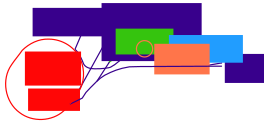
\includegraphics[width=\columnwidth]{chapter3/complex_noTev.png}
   \caption{Current operational layout of the Fermilab Accelerator Complex as of 2024. Original plot provided by R. Ainsworth, first published on Ref. \cite{rr1}, but modified for this document.}
   \label{fig:fnal}
\end{figure}

The Proton Improvement Plan II (PIP-II) is the first step in establishing the Fermilab Accelerator Complex as a multi-MW proton facility \cite{pipII1}. The near-future objective is to deliver a 1.2 MW proton beam to the Deep Underground Neutrino Experiment (DUNE) through the Long-Baseline Neutrino Facility (LBNF) \cite{dune}, still in construction. In order to meet this goal, several upgrades are being planned in the accelerator complex, including a new 800 MeV superconducting linear accelerator. The future plan for the layout of the Fermilab Accelerator Complex is shown in Fig. \ref{fig:fnalpip2}. With minimal upgrades to the Main Injector and Recycler Ring, but with a substantial overhaul of the Booster Ring, this will allow for a 50\% increase in particles per pulse intensity. Table \ref{tab:rrparams} also specifies some upgrades that will happen for the PIP-II era. Some examples include an increase of the particle per bunch intensity, a shortening of the Main Injector acceleration ramp and an increase in the Booster ramping rate. As the Recycler Ring starts to deal with higher intensities from the PIP-II upgrade, it is important to mitigate the effects of space charge as discussed in Secs. \ref{sec:resonances} and \ref{sec:sc1}. Particles along the bunch will experience space charge force leading to detuning in their betatron frequencies. Given the incoherent nature of this process, this leads to the beam having a larger tune spread in the tune diagram and having particles operate on top of resonances.

\begin{figure}[H]
   \centering
   \includegraphics[width=\columnwidth]{chapter3/complexPIPII.png}
   \caption{Future layout of the Fermilab Accelerator Complex for the Proton Improvement Plan II (PIP-II). Original plot provided by R. Ainsworth, first published on Ref. \cite{rr1}, but modified for this document.}
   \label{fig:fnalpip2}
\end{figure}

\section{\label{sec:rrgen}General Description}

The RR is a permanent magnet storage ring operating at a fixed momentum of 8.835 GeV/c equivalent to an energy of 8 GeV. The basic cell structures of this machine are FODO (Focusing Quadrupole - Drift - Defocusing Quadrupole - Drift) cells. During its conception, the need for a quick and non-expensive design spurred the idea of combining quadrupole and dipole magnets into one combined function magnet. These combined function magnets can be seen in Fig. \ref{fig:rrtunnel} as the green covered magnets on the top ring--the Recycler Ring. In order to further reduce costs and human labor during its construction, these magnets were chosen to be permanent magnets made out of a strontium ferrite \cite{rr0}. Some advantages of having permanent magnets is that there is no need for power supplies, cooling systems or power distribution cables. Consequently, these type of magnets are very stable against time and temperature. Nevertheless, the magnetic field of such magnets does degrade over time. Reference \cite{rr1} shows how the fields in RR-type magnets can degrade around 1\% after 20 years. Ultimately, this slightly changes the nominal energy in the machine. 

\begin{figure}[H]
   \centering
   \includegraphics[width=\columnwidth]{chapter3/tunnel.jpg}
   \caption{Picture of the Main Injector (blue and red magnets in the bottom) and the Recycler Ring (green magnets up top) tunnel.}
   \label{fig:rrtunnel}
\end{figure}


\cite{pipII1} \cite{rr2} \cite{fermi_rookie}

\begin{figure}[H]
   \centering
   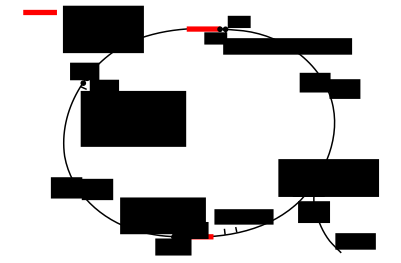
\includegraphics[width=\columnwidth]{chapter3/RRschematic.png}
   \caption{Schematic layout of the Recycler Ring and its corresponding sections. Original plot provided by R. Ainsworth, first published on Ref. \cite{rr1}.}
   \label{fig:rrschematic}
\end{figure}

\begin{table}[H]
\centering
\caption{Typical Recycler Ring properties for beam sent to NuMI}
\label{tab:rrparams}
\begin{tabular}{@{}ccc@{}}
\toprule
\textbf{Parameter}          & \textbf{Value}                             & \textbf{Unit} \\ \midrule
Circumference               & 3319.4                                     & m             \\
Momentum                    & 8.835                                      & GeV/c         \\
Revolution Period           & 11.1                                       & $\mu$s        \\
Revolution Frequency        & 90.1                                       & kHz        \\
RF Frequency                & 52.8                                       & MHz           \\
RF Voltage                  & 80                                         & kV            \\
Harmonic Number             & 588                                        &               \\
Synchrotron Tune            & 0.0028                                     &               \\
Slip Factor                 & -8.6 $\times$ 10$^{-3}$                    &               \\
Superperiodicity            & 2                                          &               \\
Horizontal Tune             & 25.43                                      &               \\
Vertical Tune               & 24.445                                     &               \\
Horizontal Chromaticity     & -6                                         &               \\
Vertical Chromaticity       & -7                                         &               \\
95\% Normalized Emittance   & 15                                         & $\pi$ mm mrad \\
95\% Longitudinal Emittance & 0.08                                       & eV s          \\
Intensity                   & $5\times10^{10}$                           & ppb           \\
                            & $8\times10^{10}$ (PIP-II)                  & ppb           \\
MI Ramp Time                & 1.2                                        & s             \\
                            & 1.133                                      & s             \\
                            & 1.067                                      & s             \\
Booster Frequency           & 15                                         & Hz            \\
                            & 20 (PIP-II)                                & Hz            \\ \bottomrule
\end{tabular}
\end{table}

\begin{figure}[H]
   \centering
   \includegraphics[width=\columnwidth]{chapter3/betas.png}
   \caption{Beta functions for the Recycler Ring lattice tuned to $Q_x=25.44$ and $Q_y=24.39$. Lattice functions calculated from lattice file using SYNERGIA.}
   \label{fig:rrbetas}
\end{figure}

\begin{equation}
   \label{eq:utotal}
   u(s) = u_{\beta}(s) + D_u(s) \delta
\end{equation}

\begin{figure}[H]
   \centering
   \includegraphics[width=\columnwidth]{chapter3/disps.png}
   \caption{Dispersion functions for the Recycler Ring lattice tuned to $Q_x=25.44$ and $Q_y=24.39$. Lattice functions calculated from lattice file using SYNERGIA.}
   \label{fig:rrdisps}
\end{figure}

\section{Tune Diagram and Resonances}

\begin{figure}[H]
   \centering
   \includegraphics[width=\columnwidth]{chapter3/rrtd.png}
   \caption{Portion of the tune diagram enclosing the operational tunes of the Recycler Ring.}
   \label{fig:rrtd}
\end{figure}

\section{High Intensity and Tune Footprint}

\begin{figure}[H]
   \centering
   \includegraphics[width=\columnwidth]{chapter3/rrtdhigh.png}
   \caption{Approximate operational tune footprint at high intensities, i.e., 1e11 particles per bunch.}
   \label{fig:rrtdhigh}
\end{figure}

\section{Diagnostic Devices}

The Recycler Ring has two main diagnostic devices that fall under the scope of this work: the Beam Position Monitors (BPMs) and the Ion Profile Monitors (IPMs). Although both systems are used to quantify properties of the beam, each one gives different information about the beam distribution. In particular, BPMs are used to probe the first moment of the transverse distribution, i.e., the mean position or beam centroid of the bunch. This is done either in one plane or in both planes simultaneously, depending on the BPM system. On the other hand, IPMs go one order higher and give information about the second order moment of the transverse beam distribution---information about the variance and spread of the bunch. Specifically for the Recycler case, there is one IPM for the horizontal direction and another one for the vertical case.

There 208 BPMs in the Recycler Ring in total. Specifically, there are 104 horizontal BPMs and 104 vertical BPMs. Each class is oriented in order to measure the corresponding plane. The BPMs are labelled according to their position around the ring as it was described in Sec. \ref{sec:rrgen} and in Fig. \ref{fig:rrschematic}. One BPM consists of two parallel pick-up electrodes that produce electric signal once the beam passes through. The beam position is determined from the relative amplitude between the signals of the opposing channels \cite{rrbpms}---also known as the $(A-B)/(A+B)$ signal. This signal is digitized and calibrated to include the scaling factors and offsets, ultimately, in order to represent the transverse beam position. The digitized signal from all 208 BPMs is interfaced to ACNET, in order to be used for accelerator applications. The resulting data is digitized every turn, hence known as turn-by-turn (TbT) data. Figure \ref{fig:bpmkick} shows an example of this TbT BPM data for a beam that was pinged in the horizontal direction recorded for 2048 turns.      

\begin{figure}[H]
   \centering
   \includegraphics[width=\columnwidth]{chapter3/bpm_kick.png}
   \caption{BPM turn-by-turn data for an arbitrary kick at horizontal BPM R:HP620.}
   \label{fig:bpmkick}
\end{figure}

One important example of using TbT data is using it in order to perform tune measurements. As mentioned in Sec. \ref{sec:basic}, specifically in Eq. \ref{eq:betatron}, the motion inside the Recycler Ring will exhibit betatron oscillations. In particular, the main harmonic of these oscillations will be dictated by the tune frequency. Say a particular set of BPM TbT data has been recorded for $N$ number of turns. Therefore, a Fast-Fourier Transform (FFT) will help uncover and measure to FFT accuracy---$\sigma_Q\approx 1/N $---the main frequency of these oscillations. Figure \ref{fig:bpmfft} shows how the main peak of the FFT can be identified in order to measure the horizontal tune $Q_x$ of the circular accelerator. Furthermore, Ch. \ref{sec:ch4} will explore how a more involved Fourier Transform algorithm, such as NAFF (Numerical Analysis of Fundamental Frequencies) will help analyze the spectrum of TbT data and measure higher order harmonics, ultimately, leading to the measurement of RDTs in the RR.     

\begin{figure}[H]
   \centering
   \includegraphics[width=\columnwidth]{chapter3/bpm_fft.png}
   \caption{Fast Fourier Transform amplitude for the turn-by-turn data presented in Fig. \ref{fig:bpmkick}.}
   \label{fig:bpmfft}
\end{figure}

\section{Elements for Resonance Compensation}

\begin{figure}[H]
   \centering
   \includegraphics[width=\columnwidth]{chapter3/sextupoles.png}
   \caption{Picture of compensation sextupoles (yellow magnets on top) installed in the Recycler Ring.}
   \label{fig:sextupoles}
\end{figure}
\chapter{Compensation of Third-Order Resonances at Low Intensities}
\label{sec:ch4}

\section{Global RDTs and Lattice Model}

\begin{table}[H]
    \centering
    \caption{Corresponding RDTs and spectral lines for each resonance line.}
    \begin{tabular}{lc}
        \toprule
        \textbf{Resonance Line} & \textbf{RDT Expression} \\
        \midrule
            $3Q_x=76$     & $\displaystyle{h_{3000} = -\frac{1}{48}\sum_i K_{2,i} L_i \beta_{x,i}^{\frac{3}{2}} e^{3i\phi_{x,i}}}$    \\ %[3pt]
           $Q_x+2Q_y=74$   &  $\displaystyle{h_{1020} = -\frac{1}{16} \sum_i K_{2,i} L_i \beta_{x,i}^{\frac{1}{2}} \beta_{y,i} e^{i \left[ \phi_{x,i} + 2\phi_{y,i}\right]} }$       \\ %[3pt]
            $3Q_y=73$     &  $ \displaystyle{h_{0030} = -\frac{1}{48}\sum_i K_{2,i}^{(s)} L_i \beta_{y,i}^{\frac{3}{2}} e^{3i\phi_{y,i}}}$ \\ %[3pt]
            $2Q_x+Q_y=75$   & $ \displaystyle{h_{2010} = -\frac{1}{16}\sum_i K_{2,i}^{(s)} L_i \beta_{x,i} \beta_{y,i}^{\frac{1}{2}} e^{i \left[ 2\phi_{x,i} + \phi_{y,i}\right]}}$       \\
        \bottomrule
    \end{tabular}
    \label{tab:rdts}
\end{table}

\begin{figure}[H]
    \centering
    \includegraphics[width=\columnwidth]{chapter4/h3000_bare.png}
    \caption{Distribution of the $h_{3000}$ term around the ring with individual contributions from each relevant element and the cumulative sum from an arbitrary starting point.}
    \label{fig:h3000bare}
\end{figure}

\begin{figure}[H]
    \centering
    \includegraphics[width=\columnwidth]{chapter4/h1020_bare.png}
    \caption{Distribution of the $h_{1020}$ term around the ring with individual contributions from each relevant element and the cumulative sum from an arbitrary starting point.}
    \label{fig:h1020bare}
\end{figure}

\section{Measurement of Third Order RDTs}

\begin{equation}
    \label{eq:hxspect}
    h_x^{-}(N)= \hat{x} \pm \hat{p}_x = \sum_{jklm}HSL_{jklm}e^{2\pi i N \left[ \left( 1-j+k\right)Q_x+\left( m-l \right)Q_y\right]}
\end{equation}

\begin{equation}
    \label{eq:hyspect}
    h_y^{-}(N)= \hat{y} \pm \hat{p}_y = \sum_{jklm}VSL_{jklm}e^{2\pi i N \left[ \left( k-j\right)Q_x+\left(1-l+m \right)Q_y\right]}
\end{equation}

\begin{multline}
    \label{eq:hxpsi2}
    h_x^{-}(N)=\sqrt{2I_x}e^{i\left( \psi_x+\psi_{x_0}\right)} \\
    -2i \sum_{jklm} j f_{jklm} \left( 2I_x \right)^{\frac{j+k-1}{2}}\left( 2I_y \right)^{\frac{l+m}{2}}
    e^{i \left[ \left( 1-j+k\right)\left( \psi_x + \psi_{x_0} \right) +\left( m-l\right)\left( \psi_y + \psi_{y_0} \right)\right]}.
\end{multline}

\begin{multline}
    \label{eq:hypsi2}
    h_y^{-}(N)=\sqrt{2I_y}e^{i\left( \psi_y+\psi_{y_0}\right)} \\
    -2i \sum_{jklm} l f_{jklm} \left( 2I_x \right)^{\frac{j+k}{2}}\left( 2I_y \right)^{\frac{l+m-1}{2}}
    e^{i \left[ \left( k-j\right)\left( \psi_x + \psi_{x_0} \right) +\left( 1-l+m\right)\left( \psi_y + \psi_{y_0} \right)\right]}.
\end{multline}

\begin{figure}[H]
    \centering
    \includegraphics[width=\columnwidth]{chapter4/hxspect.png}
    \caption{Spectral lines of $h_x^{-}$ calculated with SUSSIX \cite{sussix}. The $h_x^{-}$ signal was reconstructed for the 104 Horizontal BPMs. The spectrum for all BPMs is superimposed in this plot.}
    \label{fig:hxspect1}
\end{figure}

\begin{figure}[H]
    \centering
    \includegraphics[width=\columnwidth]{chapter4/hyspect.png}
    \caption{Spectral lines of $h_y^{-}$ calculated with SUSSIX \cite{sussix}. The $h_y^{-}$ signal was reconstructed for the 104 Vertical BPMs. The spectrum for all BPMs is superimposed in this plot.}
    \label{fig:hyspect1}
\end{figure}

\begin{table}[H]
    \centering
    \caption{Corresponding RDTs and location of spectral lines for each resonance line.}
    \begin{tabular}{lcccc}
        \toprule
        \textbf{Resonance Line} & \textbf{Source} & \textbf{RDT} & \textbf{Hor. Spect.} & \textbf{Vert. Spect.} \\
        \midrule
            $3Q_x=76$     & Normal Sextupole    & $h_{3000}$           &  (-2,0)  & -       \\ %[3pt]
           $Q_x+2Q_y=74$   & Normal Sextupole    & $h_{1020}$            & (0,-2) & (-1,-1)       \\ %[3pt]
            $3Q_y=73$     & Skew Sextupole   & $h_{0030}$           & - & (0,-2)        \\ %[3pt]
            $2Q_x+Q_y=75$   & Skew Sextupole    & $h_{2010}$     & (-1,-1) & (-2,0)       \\
        \bottomrule
    \end{tabular}
    \label{tab:rdtlines}
\end{table}

\begin{figure}[H]
    \centering
    \includegraphics[width=\columnwidth]{chapter4/bpm_kick.png}
    \caption{}
    \label{fig:bpm_kick0}
\end{figure}

\begin{figure}[H]
    \centering
    \includegraphics[width=\columnwidth]{chapter4/ellipse_data.png}
    \caption{}
    \label{fig:ellipse}
\end{figure}

\section{Compensation of RDTs}

For resonance compensation we have four dedicated normal sextupoles with currents that can be set to ($I_{sc220},I_{sc222},I_{sc319},I_{sc321}$) and four dedicated skew sextupoles with currents that can be set to ($I_{ss323},I_{ss323},I_{ss319},I_{ss321}$). As shown in the previous section one RDT can be cancelled out with the right kick from the correction elements, which means the resonances are corrected to first order. 

Nevertheless, by compensating one resonance line, other resonances  might become worse. This is why for simultaneous compensation, compensation currents will vary depending on the subsets of resonances to compensate. In principle, the currents $I_x$ needed in each correction element in order to cancel out the four bare machine RDTs, are given by the solution to this linear system of equations: 
\begin{equation}
    \begin{bmatrix}
        -|{h_{3000}}|  \cos (\psi_{3000})\\
        -|{h_{3000}}|  \sin (\psi_{3000})\\
        -|{h_{1020}}|  \cos (\psi_{1020})\\
        -|{h_{1020}}|  \sin (\psi_{1020})\\
        -|{h_{0030}}|  \cos (\psi_{3000})\\
        -|{h_{0030}}|  \sin (\psi_{3000})\\
        -|{h_{2010}}|  \cos (\psi_{1020})\\
        -|{h_{2010}}|  \sin (\psi_{1020})\\
      \end{bmatrix}_{(Bare)}
    =
      \boldsymbol{M}
    \begin{bmatrix}
        I_{sc220} \\
        I_{sc222} \\
        I_{sc319} \\
        I_{sc321} \\
        I_{ss223} \\
        I_{ss323} \\
        I_{ss319} \\
        I_{ss321} \\
      \end{bmatrix}
    \label{eq:system}
\end{equation}
where $M_{ij}$ is the response matrix for the RDTs with respect to the currents, and includes any roll that can happen for the correction sextupoles. This response matrix $M_{ij}$ can be calculated by scanning the currents in each correction element and looking at the response from the real and imaginary part of the RDTs, i.e., $h_{jklm}=|h_{jklm}|e^{i\psi_{jklm}}$. 

In reality, there are limitations to solving equation \ref{eq:system}. The first one is that all the RDTs ($h_{jklm}$) may not be accessible for measurement, given that they may not show up as a spectral line.  Another limitation is that the solution for the currents may be outside the maximum limits for the correction elements. 

One can also try to cancel out a subset of RDTs from equation \ref{eq:system}, including only one RDT. For example, in order to compensate $3 Q_x=76$, the system of equations to be solved is:

\begin{equation}
    \begin{bmatrix}
        -|{h_{3000}}|  \cos (\psi_{3000})\\
        -|{h_{3000}}|  \sin (\psi_{3000})\\
        0\\
        0\\
      \end{bmatrix}_{(Bare)}
    =
    \begin{bmatrix}
        M_{11} & M_{12} & M_{13} & M_{14} \\
        M_{21} & M_{22} & M_{23} & M_{24} \\
        1 & 1 & 0 & 0 \\
        0 & 0 & 1 & 1 \\
    \end{bmatrix}
    \begin{bmatrix}
        I_{sc220} \\
        I_{sc222} \\
        I_{sc319} \\
        I_{sc321} \\
      \end{bmatrix}
    \label{eq:system1}
\end{equation}

\begin{figure}[H]
    \centering
    \includegraphics[width=\columnwidth]{chapter4/h3000_3qxcomp.png}
    \caption{Distribution of the $h_{3000}$ term around the ring with individual contributions from each relevant element and the cumulative sum from an arbitrary starting point when correction elements are set to compensate $3Q_x=76$, i.e., $h_{3000}=0$.}
    \label{fig:h3000_3qxcomp}
\end{figure}

\begin{figure}[H]
    \centering
    \includegraphics[width=\columnwidth]{chapter4/h1020_3qxcomp.png}
    \caption{Distribution of the $h_{1020}$ term around the ring with individual contributions from each relevant element and the cumulative sum from an arbitrary starting point when correction elements are set to compensate $3Q_x=76$, i.e., $h_{3000}=0$.}
    \label{fig:h1020_3qxcomp}
\end{figure}

\section{Optimization of Compensation Currents}

\section{Experimental Verification of Compensation}

\subsection{\label{sec:lossmaps}Dynamic Loss Maps}

One effective method for visualizing resonance compensation involves constructing dynamic loss maps. To generate these representations, specialized quadrupoles responsible for controlling the tune of the Recycler are gradually adjusted to map out the desired tune area. Throughout this process, the beam loss rate is meticulously measured and interpolated across the specified region. This is done in the horizontal and vertical direction. The initial horizontal scan is generated by maintaining a constant vertical tune while implementing a horizontal tune ramp ranging from $Q_x=25.47$ to $Q_x=25.31$. Subsequently, the vertical tune, initially set as \textit{constant} at $Q_y=24.47$, is adjusted incrementally to $Q_y=24.31$ in steps of 0.005, with intensity data recorded at each step. Conversely, for the vertical scan, the roles are reversed: the horizontal tune remains constant while a vertical tune ramp progresses from $Q_y=24.47$ to $Q_y=24.31$. Then, the \textit{constant} horizontal tune is varied from $Q_x=25.47$ to $Q_y=25.31$ in steps of 0.005. The resulting intensity data from both scans can be differentiated, normalized by the instantaneous intensity, and interpolated within a two-dimensional grid to construct plots akin to those depicted in Figs. \ref{fig:bare_nocomments} and \ref{fig:bare_comments}. Figure \ref{fig:bare_nocomments} demonstrates the initial machine scan without any compensation. If plotted alongside the theoretical positions of the lines as in Fig. \ref{fig:bare_comments}, the beam loss bands align with the resonance lines. 

Figure \ref{fig:bare_comments} illustrates the correspondence between the loss patterns and the theoretical positions of resonance lines. A slight deviation exists between the set tune and the actual tune due to calibration adjustments from the tune trombone program. However, despite this variance, the resonance line configuration within the loss pattern facilitates the visualization of each resonance's strength. Specifically, a higher normalized loss at a particular tune location indicates a stronger Resonance Driving Term (RDT) for the corresponding resonance line. Within Figs. \ref{fig:bare_nocomments} and \ref{fig:bare_comments}, third, fourth, and even traces of fifth-order resonance lines are discernible, with third-order resonance lines exhibiting the greatest prominence.

Figure \ref{fig:lossmaps} depicts dynamic loss maps representing various configurations of the compensation sextupoles. Specifically, Fig. \ref{fig:sfig1} illustrates the loss map for the bare machine, where no compensation sextupoles are activated, while Fig. \ref{fig:sfig2} and Fig. \ref{fig:sfig3} demonstrate compensation for a single resonance line each. In the case of $3Q_x$ compensation, the four normal sextupoles are adjusted to the calculated compensation currents using the RDT response matrix method. Moreover, a comparison between Fig. \ref{fig:sfig2} and Fig. \ref{fig:sfig1} clearly indicates a reduction of normalized losses by two orders of magnitude at the $3Q_x$ line with compensation. This observation holds true for the $3Q_y$ compensation as well, as shown in Fig. \ref{fig:sfig3}.

Figures \ref{fig:sfig4}, \ref{fig:sfig5}, and \ref{fig:sfig6} showcase the optimal configurations of compensation sextupoles designed to address multiple resonance lines simultaneously. It's important to note that while attempting to compensate for one or multiple resonance lines, there's a possibility that other resonance lines may strengthen. This is evident in the explicit case depicted in Fig. \ref{fig:sfig6}, where compensating for $3Q_y$ and $Q_x+2Q_y$ leads to the amplification of the $2Q_x+Q_y$ resonance. Such occurrences pose a limitation when aiming to compensate for more than two resonance lines, as the compensation currents tend to increase. There exists a constraint on the currents supplied to the compensation sextupoles. For instance, in compensating both normal sextupole lines, $3Q_x$ and $Q_x+2Q_y$, the required currents exceed the current limit. Ongoing efforts are focused on reducing the compensation currents in this specific scenario. Section \ref{sec:addsexts} summarizes some of these efforts, where additional sextupoles have been installed in order to decrease the currents that cancel out both the $h_{3000}$ and $h_{1020}$ RDTs.

Another notable detail evident in Figs. \ref{fig:sfig1}-\ref{fig:sfig6} is the presence of white areas within the loss maps, indicating regions where there was insufficient beam to accurately map out the losses. In certain configurations of the compensation sextupoles, the combined weakening of the third-order resonance lines occurs in a manner that leaves some beam remaining beyond these lines. It could be argued that conducting two additional scans, injecting from the left and bottom, could effectively map out these inaccessible regions. Such an enhancement could be considered as a future upgrade to these dynamic loss maps. Ultimately, all the plots presented in Fig. \ref{fig:lossmaps} demonstrate various potential configurations that open up regions of tune space for utilization during operations, enabling the accommodation of high-intensity beams.

\begin{figure}[H]
    \centering
    \includegraphics[width=\columnwidth]{chapter4/bare.png}
    \caption{Dynamic loss map from ramping the tunes with an interval of $\Delta Q_u=0.005$ in both directions. The directions of scan are from left to right and top to bottom. The results are superimposed in this plot.}
    \label{fig:bare_nocomments}
\end{figure}

\begin{figure}[H]
    \centering
    \includegraphics[width=\columnwidth]{chapter4/bare_comments.png}
    \caption{Dynamic loss map with the corresponding lines from Fig. \ref{fig:rrtd} drawn on top.}
    \label{fig:bare_comments}
\end{figure}


\newpage
\begin{figure}[H]

    \centering
    \begin{subfigure}{.49\textwidth}
      \includegraphics[width=0.98\linewidth]{chapter4/bare.png}
      \caption{Bare machine}
      \label{fig:sfig1}
    \end{subfigure}%
    \hfill
    \begin{subfigure}{.49\textwidth}
      \includegraphics[width=0.98\linewidth]{chapter4/3qx.png}
      \caption{$3Q_x$ Compensation}
      \label{fig:sfig2}
    \end{subfigure}
    \hfill
    \begin{subfigure}{.49\textwidth}
      \includegraphics[width=0.98\linewidth]{chapter4/3qy.png}
      \caption{$3Q_y$ Compensation}
      \label{fig:sfig3}
    \end{subfigure}
    \hfill
    \begin{subfigure}{.49\textwidth}
      \includegraphics[width=0.98\linewidth]{chapter4/3qx_3qy.png}
      \caption{$3Q_x$ and $3Q_y$ Compensation}
      \label{fig:sfig4}
    \end{subfigure}%
    \hfill
    \begin{subfigure}{.49\textwidth}
      \includegraphics[width=0.98\linewidth]{chapter4/3qx_2qxqy.png}
      \caption{$3Q_x$ and $2Q_x+Q_y$ Compensation}
      \label{fig:sfig5}
    \end{subfigure}
    \hfill
    \begin{subfigure}{.49\textwidth}
      \includegraphics[width=0.98\linewidth]{chapter4/3qy_qx2qy.png}
      \caption{$3Q_y$ and $Q_x+2Q_y$ Compensation}
      \label{fig:sfig6}
    \end{subfigure}
    
    \caption{Dynamic loss maps for several configurations of compensation sextupoles}
    \label{fig:lossmaps}
    \end{figure} 
\newpage


\subsection{Static Tune Scans}

Another method for visualizing resonance compensation involves static tune scans. While the loss maps detailed earlier illustrate the dynamic crossing of resonance, an alternative method entails setting the tune to a specific value and assessing the beam survival ratio alongside the beam size over a defined time interval. The beam size is quantified using the Ion Profile Monitor System (IPM) within the ring, and the results are expressed in arbitrary units to indicate a relative effect.

\begin{figure}[H]
    \centering
    \includegraphics[width=\columnwidth]{chapter4/static2turns.png}
    \caption{Static tune scan for bare machine with comparisons between experimental data and SYNERGIA simulations.}
    \label{fig:static2}
\end{figure}

% \begin{figure}[H]
%     \centering
%     \includegraphics[width=\columnwidth]{chapter4/static2turns_comp.png}
%     \caption{Plot for static tune scan for machine with $3Q_x$ compensation including comparison between experimental data and SYNERGIA simulations.}
%     \label{fig:static2_comp}
% \end{figure}

\begin{figure}[H]
    \centering
    \includegraphics[width=\columnwidth]{chapter4/static2turns_ipm.png}
    \caption{Static tune scan with beam survival ratio and IPM data box plots for bare machine at 2 Booster Turns of equivalent intensity.}
    \label{fig:static2_ipm}
\end{figure}

\begin{figure}[H]
    \centering
    \includegraphics[width=\columnwidth]{chapter4/static2turns_comp_ipm_dampersOFF.png}
    \caption{Static tune scan with beam survival ratio and IPM data box plots for machine with $3Q_x$ compensation at 2 Booster Turns of equivalent intensity.}
    \label{fig:static2_ipm_comp}
\end{figure}

\section{Additional Sextupoles for Resonance Compensation}
\label{sec:addsexts}

\begin{equation}
    \begin{bmatrix}
        -|h_{3000}| \cos \psi_{3000} \\
        -|h_{3000}| \sin \psi_{3000} \\
        -|h_{1020}| \cos \psi_{1020} \\
        -|h_{1020}| \sin \psi_{1020} \\
        \end{bmatrix}_{(Bare)}
         =
        \boldsymbol{M}
        \begin{bmatrix}
        k_2^{(sc220)} \\
        k_2^{(sc222)}\\
        k_2^{(sc319)} \\
        k_2^{(sc321)}\\
        \end{bmatrix}
        \label{eq:systemk2s}        
\end{equation}

\begin{figure}[H]
    \centering
    \includegraphics[width=\columnwidth]{chapter4/old_config_h3000.png}
    \caption{Distribution of the $h_{3000}$ term around the ring with individual contributions from each relevant element and the cumulative sum from an arbitrary starting point. This is with existing sextupoles powered at the correct currents to cancel out $h_{3000}$ and $h_{1020}$ simultaneously.}
    \label{fig:h3000oldconfig}
\end{figure}

\begin{figure}[H]
    \centering
    \includegraphics[width=\columnwidth]{chapter4/old_config_h1020.png}
    \caption{Distribution of the $h_{1020}$ term around the ring with individual contributions from each relevant element and the cumulative sum from an arbitrary starting point. This is with existing sextupoles powered at the correct currents to cancel out $h_{3000}$ and $h_{1020}$ simultaneously.}
    \label{fig:h1020oldconfig}
\end{figure}

\begin{equation}
    \begin{bmatrix}
        -|h_{3000}| \cos \psi_{3000} \\
        -|h_{3000}| \sin \psi_{3000} \\
        -|h_{1020}| \cos \psi_{1020} \\
        -|h_{1020}| \sin \psi_{1020} \\
        \end{bmatrix}_{(Bare)}
         =
        \boldsymbol{M}
        \begin{bmatrix}
        k_2^{(sc220)} \\
        k_2^{(sc222)}\\
        k_2^{(sc319)} \\
        k_2^{(sc321)}\\
        k_2^{(1)} \\
        k_2^{(2)}\\
        \end{bmatrix}
        \label{eq:systemadd}
\end{equation}

\begin{figure}[H]
    \centering
    \includegraphics[width=\columnwidth]{chapter4/new_sexts_dx.png}
    \caption{Dispersion function of the Recycler Ring with possible new locations to introduce a pair of sextupole magnets that cancel out $h_{3000}$ and $h_{1020}$ simultaneously. The right y-axis shows the maximum compensation current needed with these new candidates.}
    \label{fig:dxnewsexts}
\end{figure}

\begin{figure}[H]
    \centering
    \includegraphics[width=\columnwidth]{chapter4/new_sexts_h3000.png}
    \caption{Distribution of the $h_{3000}$ term around the ring with individual contributions from each relevant element and the cumulative sum from an arbitrary starting point. This is with the new 620 sextupoles powered at the correct currents to cancel out $h_{3000}$ and $h_{1020}$ simultaneously.}
    \label{fig:h3000newsexts}
\end{figure}

\begin{figure}[H]
    \centering
    \includegraphics[width=\columnwidth]{chapter4/new_sexts_h1020.png}
    \caption{Distribution of the $h_{1020}$ term around the ring with individual contributions from each relevant element and the cumulative sum from an arbitrary starting point. This is with the new 620 sextupoles powered at the correct currents to cancel out $h_{3000}$ and $h_{1020}$ simultaneously.}
    \label{fig:h1020newsexts}
\end{figure}

\chapter{Resonance Compensation Studies at the CERN Proton Synchrotron Booster}
\label{sec:ch5}

\section{General specifications}

\section{Tune Diagram and Operation}

\section{Optimization Algorithms for Resonance Compensation}

\section{Experimental Verification of Compensation}

\chapter{Conclusions and Future Work}
\label{sec:ch6}

\chapter{Conclusions and Future Work}
\label{sec:ch7}

The work shown throughout this document can also be found in Refs. \cite{cris1,cris2, cris3}. This section reports on the conclusions and future work stemming from this thesis.

\section{Conclusions}

\subsection{RDTs and Resonance Compensation}

The measurement and subsequent cancellation of RDTs was investigated in depth in Ch. \ref{sec:ch4}. It was shown that third order RDTs in the Recycler Ring can be measured and, afterwards, cancelled with the compensation sextupoles in place. Furthermore, optimization procedures have been developed in order to have this compensation   

\subsection{Physics-Informed vs. Optimization-Based Compensation}

Chapters \ref{sec:ch4} and \ref{sec:ch5} showed two different approaches to the same problem of resonance compensation. The first one performed at the Fermilab Recycler Ring showed how to implement the response matrix approach, which can be traced to some underlying physics principles. On the other hand, Ch. \ref{sec:ch5} shows how to implement numerical optimization algorithms for compensating multiple resonance lines at the CERN PS Booster. Nevertheless, this last approach had no direct physics input. The distinction between a physics-informed approach and a numerical-optimization approach summarizes the differences between both chapters. The 

\subsection{High-Intensity Resonance Compensation}

For current operations of the Fermilab Accelerator Complex, the third-order resonance compensation scheme developed in this work will not have an effect on reducing losses in the Recycler Ring. The current tune spreads in the RR are not large enough for the third order resonances to be specially harmful to operations. The beam coming out of Booster grows exponentially with the beam intensity, as it was shown in Fig. \ref{fig:tunespread}. Thus, saturating the tune spread at values close to 0.02---not particularly large. The losses in the Recycler Ring are purely emittance-dominated for current operations. They are not related to space charge effects. Nonetheless, the resonance compensation scheme still is beneficial to operations at high intensities. This is if the operational tune is moved closer to the third order resonance lines, which is not suggested.  

\subsection{Transverse Dampers and High-Intensity Compensation}

Section \ref{sec:ch6dampers} showed how the transverse dampers have an effect on the resonance compensation scheme. Figure \ref{fig:dampers7} reinforces this statement by showing the beam survival ratio at a high intensity of 4.5e10 ppb without compensation and dampers on(bare machine), with compensation and dampers on, and with compensation and dampers off. Ultimately, the dampers degrade the quality of the compensation. In particular, when turned off, the overall beam survival ratio increases. The configuration of the dampers---gain and phase of feedback---has been optimized away from the resonance lines. When the tunes are set close to the third order resonance lines, the dampers settings will create beam size growth. They are not optimized to run in this region, and will cause harmful effects on the beam, even with the resonance compensation scheme enabled.

\begin{figure}[H]
    \centering
    \includegraphics[width=\columnwidth]{chapter7/dampers_config.png}
    \caption{Transverse damper effect on resonance compensation for bare machine + dampers ON, $3Q_x$ compensated + dampers ON, and $3Q_x$ compensated + dampers OFF configuration. The red band corresponds to the $3Q_x$ stop band at an intensity of 0.5 ppb with dampers ON.}
    \label{fig:dampers7}
\end{figure}

\section{Future Work}

\subsection{Verification of Newly-Installed Sextupoles}

Section \ref{sec:compensate} explained the motivation behind installing additional sextupoles that would bring down that currents needed to compensate $3Q_x=76$ and $Q_x+ 2Q_y = 74$. Subsequently, Sec. \ref{sec:addsexts} explained the procedure used in order to pin down the new locations for two new compensation sextupoles. There is still future work to be done regarding the commissioning and connection of the new 620 sextupoles. The sextupoles and their power supplies need to be interfaced with ACNET. Furthermore, the resonance compensation enhancement still needs to verified by means of performing an RDT scan. Specifically, the response matrix coefficients corresponding to these new sextupoles need to be measured and calculated. All of this, following the procedure outlined in Secs. \ref{sec:rdtmeasure} and \ref{sec:compensate}. Figure \ref{fig:new620sexts} shows a picture of the newly installed sextupoles.

\begin{figure}[H]
    \centering
    \includegraphics[width=\columnwidth]{chapter7/620_sext.jpg}
    \caption{Newly installed compensation sextupoles in the 620 section.}
    \label{fig:new620sexts}
\end{figure}

\subsection{Resonances and Transverse Dampers at High Intensities}

It was shown in Sec. \ref{sec:ch6dampers} that the transverse dampers in the Recycler Ring can interact with betatron resonance lines depending on their configuration. It would be interesting to perform experiments with the configuration of these dampers in order to fully characterize these effects. Furthermore, it would also be interesting to use the dampers as anti-dampers in order to sustain betatron oscillations. With this configuration, one could perform tune measurements, and perhaps evaluate this alternative method to measure RDTs. This would be similar to having an AC dipole installed in the Recycler.  

\subsection{Effect of MI Ramp on RDTs}

The ultimate objective of this work is to have this resonance compensation scheme fully characterized in order to incorporate it into high intensity operations. Nevertheless, there is one additional factor that has been identified to also play a role in this effort. This one stems from the fact that the Main Injector and the Recycler Ring share the same tunnel. It has been shown that the acceleration ramp changes the beam dynamics inside the Recycler Ring. In particular, it introduces orbit distortions and tune shifts depending on the position of the ramp \cite{mionrr}. There is an ongoing effort in order to characterize any higher order magnetic effect from the MI to RR, e.g., any sextupole term that is being introduced by the MI acceleration ramp. The first results have shown that the compensation currents change depending on the location of the study event with respect to the MI acceleration ramp. Therefore, in the future, the resonance compensation described hereinabove should be modified to accommodate this effect to be fully operational.

\subsection{Limits of Resonance Compensation}

\subsection{Space Charge RDTs}

Equation \ref{eq:hfinal} shows how the lattice elements and the space charge potential drive betatron resonances. It would be interesting to explore further how to measure space charge resonance driving terms (SCRDTs) and their effect on the operation of the Recycler Ring. Without taking into account any collective instabilities, the ultimate limit of the Recycler Ring will be dictated by how strong these third order lines become in the space-charge dominated regime. The current future of the Main Injector and Recycler Ring lies in high-intensity beam. As the space charge potential grows for the Fermilab beams, it is important to quantify all effects from high intensity operation---being SCRDTs one of them.

\printbibliography
%\chapter{Your first chapter}
%
% If you have pages that must appear in landscape mode, use the [lscape] documentclass option
% and enclose the pages in a {landscape} environment.
%\clearpage\pagestyle{lscape} % first clear the page and change the pagestyle
%\begin{landscape}
%
% your landscape table(s) or figure(s) here
%
%\end{landscape}
%\pagestyle{plain} % remember to change the pagestyle back to plain
%
%
% Your bibliography command here 
% e.g. \bibliography{your-bib-file}) if using natbib
% e.g. \printbibliography if using biblatex
%
% Remember that although the bibliography is single spaced, there needs to
% be a blank line between entries. This is set by your bibliography package
% If you are using natbib it is \bibsep; if using biblatex it's \bibitemsep
% These are set automatically by the class if you are using these packages
%
% If you need per-chapter bibliographies, you need to use the [chapterbib]
% class option and you would use \makebibliographypage before each
% chapter level bibliography and then the relevant bibliography command
% You should not use the \backmatter command 
%
% If you have appendices, they would go here.  
% If you only have one appendix it will look like this: (comment this out if you have no appendices)
% \begin{appendices}
% \chapter{\label{sec:app1}Lie Algebra Methods for Accelerator Physics in 2D using MATHEMATICA}
\includepdf[pages=-]{lie2D.pdf}
% \chapter{\label{sec:app2}Lie Algebra Methods for Accelerator Physics in 4D using MATHEMATICA}
\includepdf[pages=-]{lie4D.pdf}
% \end{appendices}
%
%
% If you have more than one appendix, you need to use 
%   \begin{appendices}
%   \chapter{First appendix}
%   \chapter{Second appendix}
%   \end{appendices}
%
% If each chapter has its own set of appendices, then load the class with the [chapterapp] option
% and put your {appendix} or {appendices} environments at the end of each chapter.
%
%
% Even though it is very unintuitive, per-chapter appendices are STILL \chapter commands
% in your document!  If you use \section it will not work properly.
% 
% You should not use the \backmatter command 
\end{document}

